\subsection{Installing racket}

\begin{frame}[fragile]{Using an installer}
  Visit \url{https://download.racket-lang.org}. Choose your appropriate
  platform/os and click on the blue download button:

\begin{figure}[htpb]
  \centering
  \href{https://download.racket-lang.org}{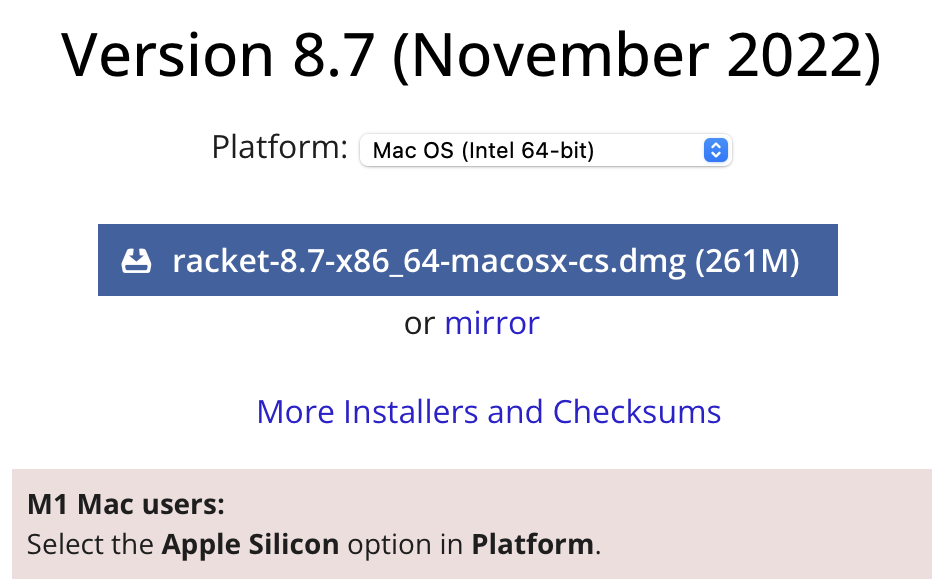
\includegraphics[width=0.5\textwidth]{./figures/official-website_racket.png}}
  \caption{Racket Official Website}
\end{figure}

For Linux operating system, the latter provides a shell script which will
install the necessary files in your system.

\end{frame}

\begin{frame}[fragile]{(Optional) Using the script for Linux}
  \begin{itemize}
  \item Execute the command \verb|sh racket-8.7-x86_64-linux-cs.sh|
  \item (Suggested) Indicate 'no' if asked 'Do you want a Unix-style
    distribution?' This allows us to specify a location to install the files.
  \item (Suggested) Indicate option 4 to install racket.
  \item Press enter to accept defaults.
  \end{itemize}
  
\end{frame}

\begin{frame}[fragile]{Using a package manager}
  \begin{itemize}
  \item For MacOs: \verb|brew install --cask racket|
  \item For Linux:
    \begin{itemize}
    \item Debian/Ubuntu:
      \verb|sudo add-apt-repository ppa:plt/racket|
      \verb|sudo apt-get install racket|
    \item Arch Linux: \verb|sudo pacman -S racket|
    \item Fedora: \verb|sudo dnf install racket|
    \item openSUSE: \verb|sudo zypper install racket|
    \end{itemize}
  \end{itemize}
\end{frame}